\chapter{Modelling of a circulating channel}


 In this chapter, the modelling work of a circulating channel based on the same bubbly flow model discussed in the previous chapter will be presented. First, the model setup will be introduced; then, we will do a parametric study by changing the channel width and the current density, so that we can analyze how these parameters impact the flow behaviour. 
 
 
\section{Model setup}

In the vertical channel geometry, we have tested the bubbly model and the relating slip models and known that it could reproduce the results from the experiment and other simulations from literature. In this section, we will implement the same bubbly flow model tested before in the circulating channel, with the same material properties presented in table \ref{materialpropeties}. 


\subsection{Geometry}
The circulating channel presented in this section belongs to natural circulating flow, in which the flow is completely driven by the gas evolution along the electrode. Figure \ref{circulatingchannel} gives a sketch of it.


As we can see, the gas is injected from the vertical electrode at the right-hand side of the channel, and with the free surface at the top boundary, the evolved gas can leave the computation domain freely while the liquid is trapped inside and circulating. After the model reaches a steady-state, the riser part is similar to the vertical channel presented in the previous chapter.

The geometry parameter is given in table \ref{geometrypropeties}:

\begin{table}[h!]
\centering
\caption{Geometry of circulating channel}
\label{geometrypropeties}
\begin{tabular}{l  l| l  l}
\hline
    $M$  & $0.1 \, \mathrm{m}$ & $D$ & $0.05\, \mathrm{m}$ \\
\hline
    $N$  & $0.1\, \mathrm{m}$  & $W$ & $0.01\, \mathrm{m}$ \\
\hline
    $L$ & $0.075\, \mathrm{m}$ & $H$ & $0.2\, \mathrm{m}$ \\
\hline
\end{tabular}
\end{table}

Note that in table \ref{geometrypropeties}, while the rest of the geometry parameter is fixed, $W$ will be varying in the parametric study.



\subsection{Boundary conditions}

Gas is evolved along the electrode:
\begin{equation}
    N_{gas}(x = D+L+W) = -\frac{RTi_{av}}{2pF}, \quad for \quad N \leq y \leq N+H
\end{equation}

At the top boundary is the free surface, for gas phase, it is pressure outlet, while for liquid phase it is a wall with free slip:

\begin{equation}
    \frac{du_{dy}(y = N+H+M)}{dy} = 0
\end{equation}
\begin{equation}
    u_{cy}(y = N+H+M) = 0 
\end{equation}

\begin{equation}
    \frac{du_{cx}(y = N+H+M)}{dx} = 0 
\end{equation}

The pressure is fixed to atmospheric pressure at the top boundary with hydrostatic pressure throughout the computation domain as the initial value:

\begin{equation}
    p(y = N+H+M) = 10^5 \, \mathrm{Pa}
\end{equation}

\begin{figure}[H]
    \centering
    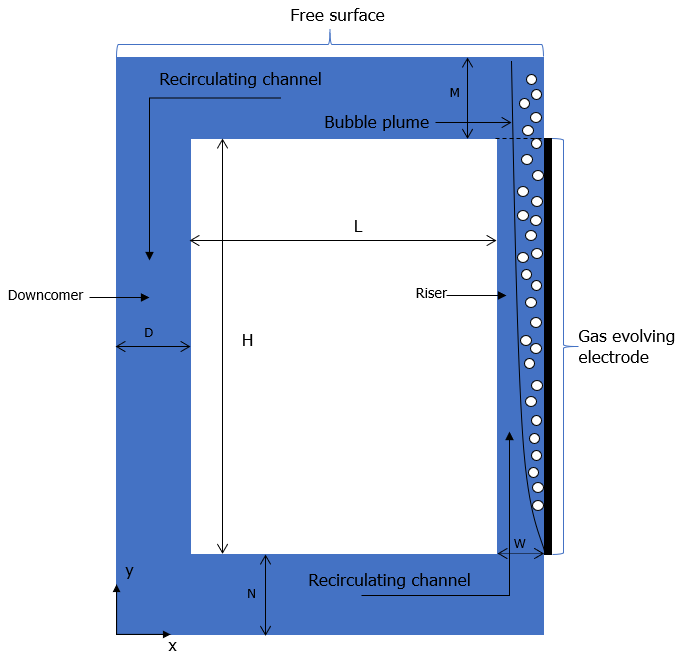
\includegraphics[scale=1]{recirculatingchannel.png}
    \caption{A sketch for the circulating channel}
    \label{circulatingchannel}
\end{figure}


\subsection{Meshing}

Figure \ref{Meshcirculating} gives the mesh used in this study. Similar to the model presented in the previous chapter, structured mesh with quadrilateral elements is also used for the circulating channel. The mesh in the riser is more refined than elsewhere, and the mesh near the wall in the riser is further refined.
\begin{figure}[H]
    \centering
    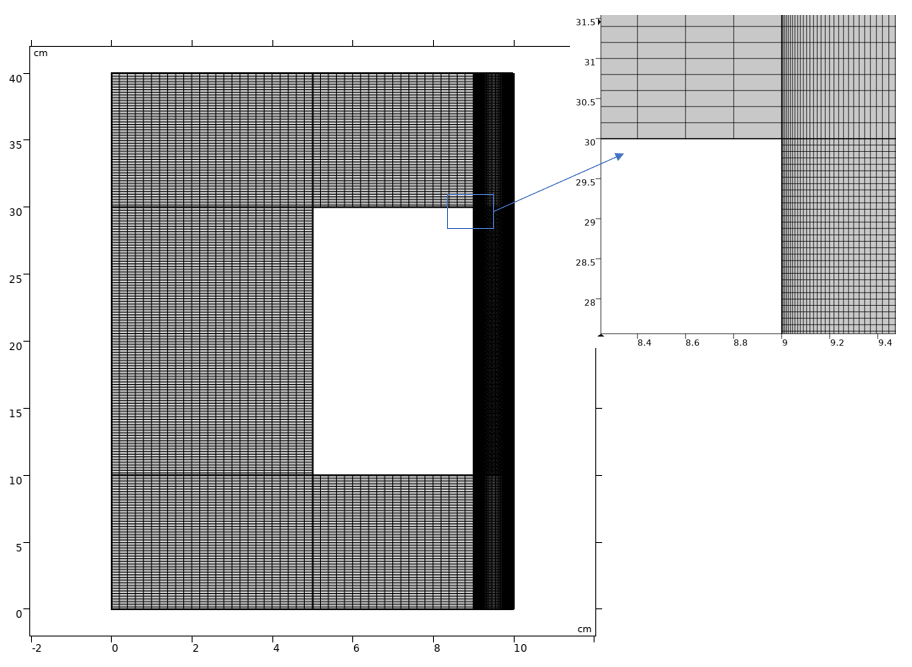
\includegraphics[scale = 0.8]{meshcirculatingchannel.png}
    \caption{The mesh for the circulating channel, the riser channel is meshed as $60 \times 200$ with the near-wall region more refined, in the remaining part the mesh sizes are all $2 \, \mathrm{mm} \times 2 \, \mathrm{mm}$}
    \label{Meshcirculating}
\end{figure}

 
 \section{Results}
 
In this section, we present the results from the simulation of a circulating channel. First, we give an overview of the results by giving a 2D contour of velocity in a typical circulating channel with a $1\, \mathrm{cm}$ riser channel gap in figure \ref{velocitycontour}. Figure \ref{velocityprofilecirculating} and figure \ref{volumefractionprofilecirculating} give the velocity and volume fraction profile across the channel at different heights. 

From these figures, we can see several aspects worth further analysis:

\begin{itemize}
    \item Velocity is significantly higher in the near-wall region. This is because the gas evolved there could drive the flow upwards. However, as channel width decreases this effect also gradually fades, and the velocity profile is close to Poiseuille flow in a narrow channel (channel width $W < 0.2 \, \mathrm{cm}$)
    \item Backflow exists in the channel as the channel width increases, which implies a relation between the backflow and input parameters like current density and channel width can be derived from the model.
    \item Analytical solutions could be derived to estimate the circulating velocity in the channel.
    \item Based on the volume fraction profile, we can see there is a plume formed in the near-wall region. The influence of input parameters on the plume thickness would be worth investigation.
\end{itemize}



 \begin{figure}[H]
     \centering
     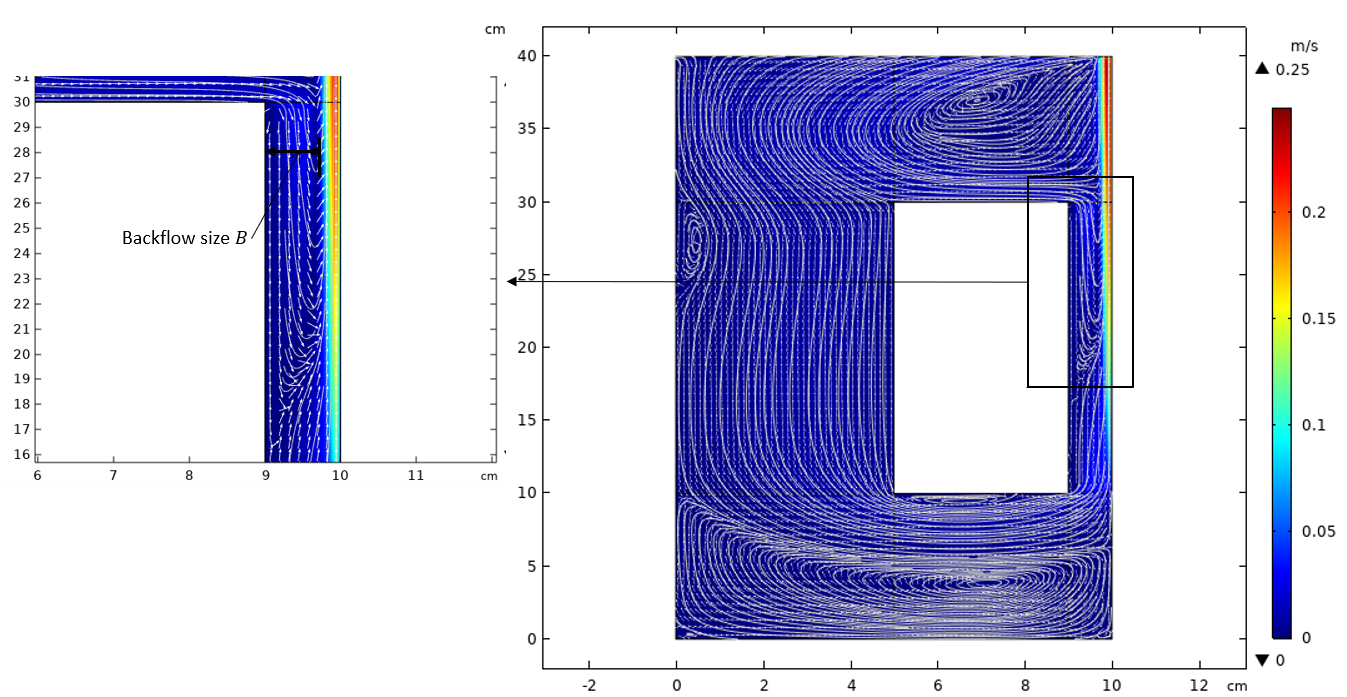
\includegraphics[scale=0.6]{velocitycontour.png}
     \caption{The 2D velocity contour in a circulating channel, the legend stands for the magnitude of velocity, the riser channel width is $1 \, \mathrm{cm}$, and the average current density is $1000 \, \mathrm{A/m^2}$, backflow can be observed in the zoomed in region}
     \label{velocitycontour}
 \end{figure}
 
 \begin{figure}[H]
     \centering
     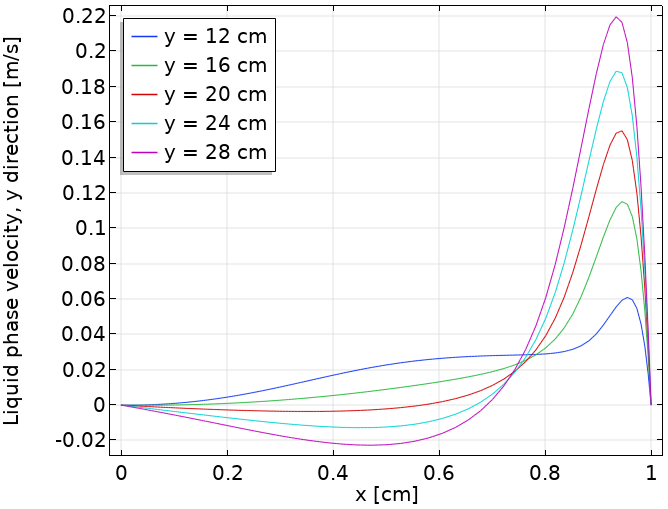
\includegraphics[scale = 0.7]{velocityprofile1cm1000A.png}
     \caption{The velocity profiles across the channel at different heights in a $1 \, \mathrm{cm}$ riser channel, $i_{av} = 1000 \, \mathrm{A/m^2}$}
     \label{velocityprofilecirculating}
 \end{figure}
 
 
 \begin{figure}[H]
     \centering
     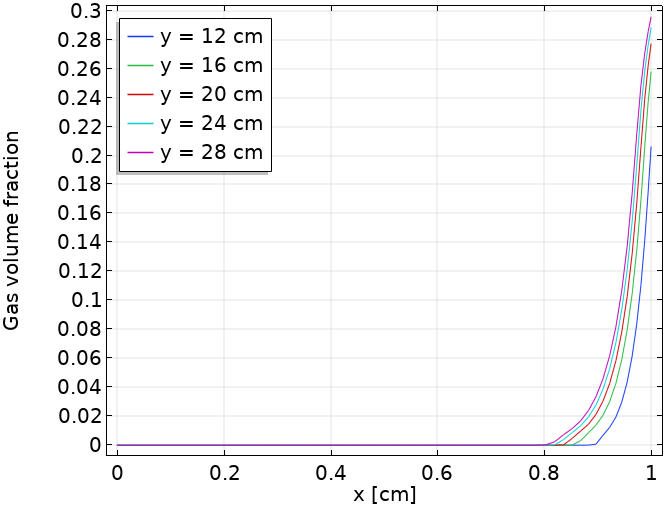
\includegraphics[scale = 0.7]{volumefraction1cm1000A.png}
     \caption{The volume fraction profiles across the channel at different heights in a $1 \, \mathrm{cm}$ riser channel, $i_{av} = 1000 \, \mathrm{A/m^2}$}
     \label{volumefractionprofilecirculating}
 \end{figure}
 
 

 
 
 \subsection{Mesh dependence study}
 
    \begin{figure}[H]
     \centering
     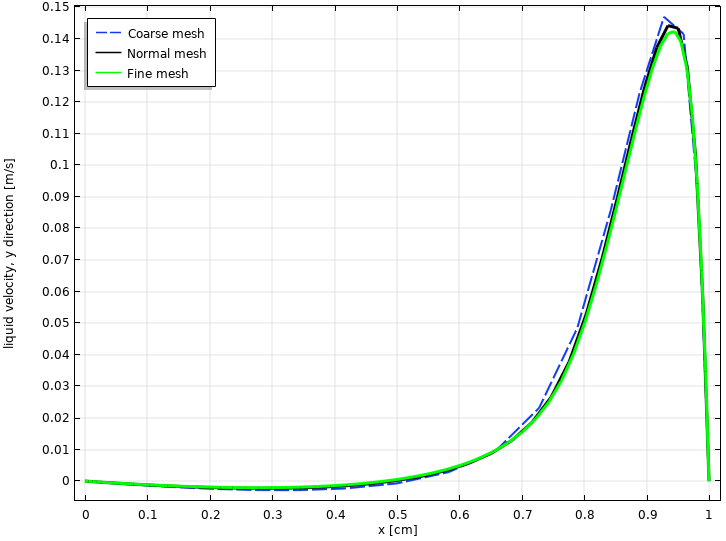
\includegraphics[scale = 0.7]{meshdependencecirculating.png}
     \caption{The mesh dependence study, the results are chosen at $y = 20 \, \mathrm{cm}$. In the riser channel, coarse mesh: $20 \times 100$, normal mesh: $40 \times 200$, fine mesh: $60 \times 300$. Outside the riser channel mesh sizes are the same.}
     \label{meshdependececirculating}
 \end{figure}
 
 Before diving into the parametric study, we need to make sure the solution obtained is mesh-independent, and use the mesh with the best balance between the computation cost and accuracy to get the results faster. A velocity profile across the channel at $y = 20 \, \mathrm{cm}$ is given in figure \ref{meshdependececirculating} as an evaluation of mesh dependence. As we can see, the solutions between $40 \times 200$ and $60 \times 300$ are nearly the same; thus, the former mesh is chosen as the one used for parametric study for shorter simulation time.
 


\section{Parametric study}

In the previous section, the velocity and volume fraction profile in a $1 \, \mathrm{cm}$ channel have been presented; now, we can tune the channel gap, current density and slip model to gain more insights.
\subsection{Volume fraction profile}

\paragraph{Volume fraction profile with and without Saffman lift force}
\*



\begin{figure}[H]
\centering
\begin{subfigure}{.5\textwidth}
  \centering
  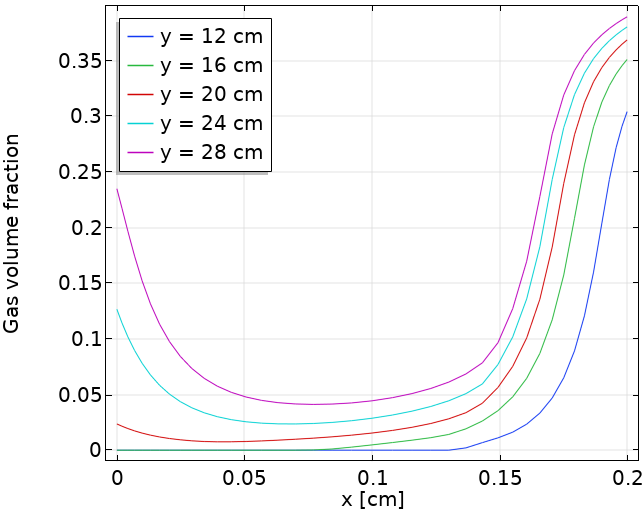
\includegraphics[width=1\linewidth]{volumefraction2mm1000A.png}
  \caption{The volume fraction profiles in a 0.2 cm channel, $i_{av}=1000 \, \mathrm{A/m^2}$}
\end{subfigure}%
\begin{subfigure}{.5\textwidth}
  \centering
  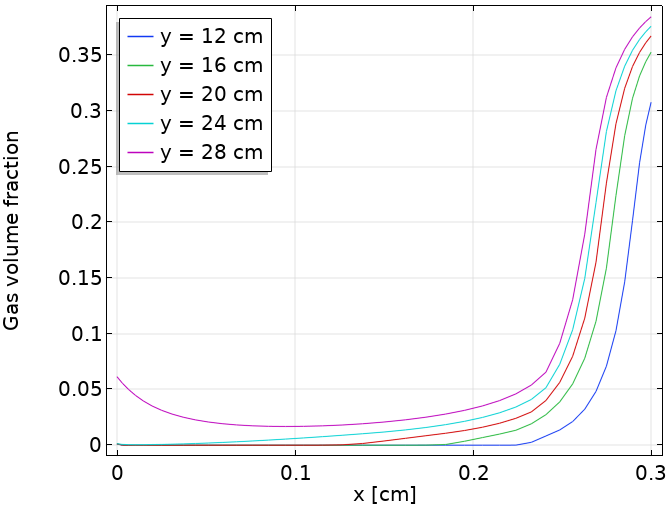
\includegraphics[width=1\linewidth]{volumefraction3mm1000A.png}
  \caption{The volume fraction profiles in a 0.3 cm channel, $i_{av}=1000 \, \mathrm{A/m^2}$}
\end{subfigure}
\begin{subfigure}{.5\textwidth}
  \centering
  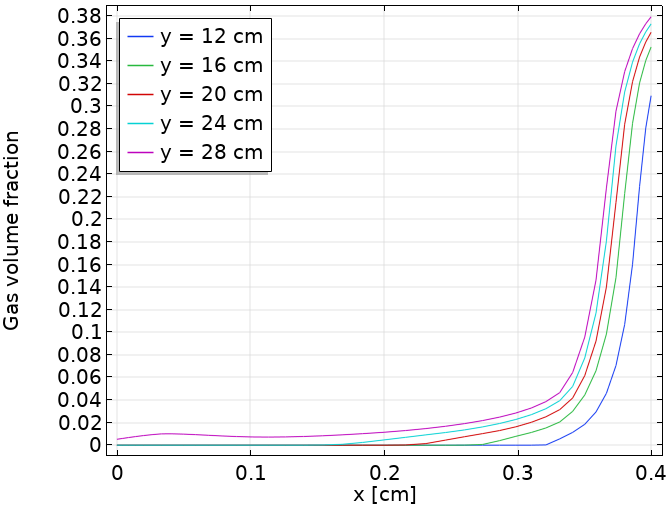
\includegraphics[width=1\linewidth]{volumefraction4mm1000A.png}
  \caption{The volume fraction profiles in a 0.4 cm channel, $i_{av}=1000 \, \mathrm{A/m^2}$}
\end{subfigure}%
\begin{subfigure}{.5\textwidth}
  \centering
  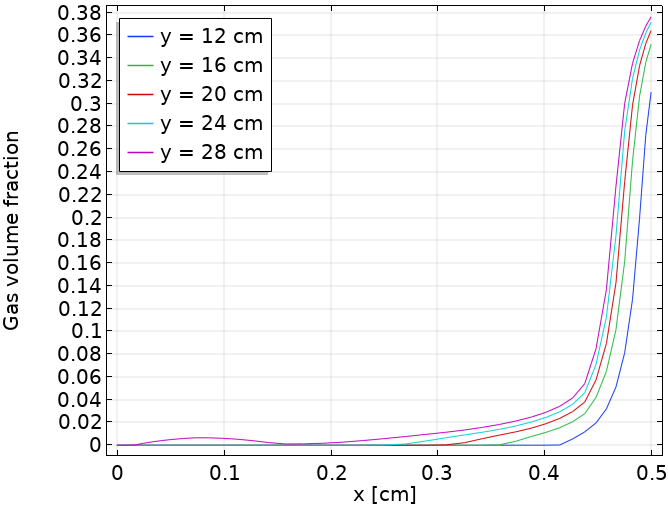
\includegraphics[width=1\linewidth]{volumefraction5mm1000A.png}
  \caption{The volume  fraction profiles in a 0.5 cm channel, $i_{av}=1000 \, \mathrm{A/m^2}$}
\end{subfigure}
\caption{The volume fraction profiles in channels with different width $W$ including the Saffman lift force, in each of the figures there are 5 profiles obtained at 5 different heights, $y = 12 \, \mathrm{cm}$, $y = 16 \, \mathrm{cm}$, $y = 20 \, \mathrm{cm}$, $y = 24 \, \mathrm{cm}$, $y = 28 \, \mathrm{cm}$}
\label{volumedifferentchannel}
\end{figure}

Figure \ref{volumedifferentchannel} gives the volume fraction profiles in different channels. From the figure, we can see that the volume fraction tends to increase on the left-hand side of the channel. After testing the slip models, we found that this effect was caused by the Saffman lift force. As discussed in Chapter 2, the Saffman lift force is based on shear rate; in this case, for narrower channels, the shear rate at the right-hand side of the channel is negative, which applies a rightward force to the bubbles forcing them to be trapped in the near-wall region. However, for some bubbles that manage to reach the other side, based on the Saffman lift force theory, they will experience a leftward force that pushes them to the other side of the channel. This Saffman lift force model is used in various models \cite{Wetind2001, Dahlkild2001, Schillings2015}, but there are actually four criteria for the correlation proposed by Saffman et al. \cite{saffman1965lift}:

\begin{equation}\label{eq:shear}
    \mathrm{R_{G}}  = \frac{|du_{ly}/dx|D_e^2}{\nu_c} \ll 1
\end{equation}

\begin{equation}
    \mathrm{R_{s}} = \frac{|\mathbf{u_{slip}}|D_e}{\nu_c} \ll 1
\end{equation}

\begin{equation}
    \mathrm{R_{O}} = \frac{|\nabla \times \mathbf{u_c}|D_e^2}{\nu_c} \ll 1
\end{equation}

\begin{equation}
    \epsilon = \frac{\mathrm{R_{G}}}{\mathrm{R_{s}}} \gg 1
\end{equation}

From the simulation, the local shear rate $|du_{ly}/dx|$ could rise up to 1000, which makes the local $R_{G} \sim 10$, which does not conform to equation \ref{eq:shear}. 

Therefore, the results without the Saffman lift force are also tested, as shown in figure \ref{nosaffvolume}.

From figure \ref{nosaffvolume}, we can see that with the Saffman lift force excluded from the model, no bubble is entrained in the left-hand side of the wall anymore. This way, the volume fraction profile seems more physical, as no pattern similar to figure \ref{volumedifferentchannel} has been found. For this reason, the analysis afterward will be done based on the model without the Saffman lift force by default.



\begin{figure}[H]
\centering
\begin{subfigure}{.5\textwidth}
  \centering
  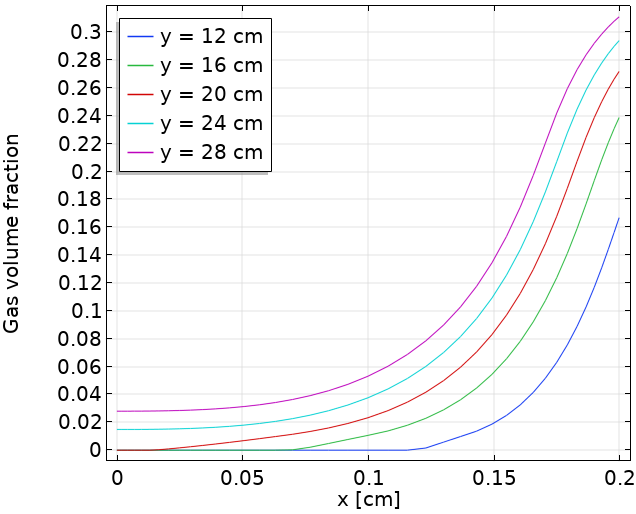
\includegraphics[width=1\linewidth]{volumefraction2mm1000Anosaff.png}
  \caption{The volume fraction profiles in a $0.2 \, \mathrm{cm}$ channel, $i_{av}=1000 \, \mathrm{A/m^2}$}
\end{subfigure}%
\begin{subfigure}{.5\textwidth}
  \centering
  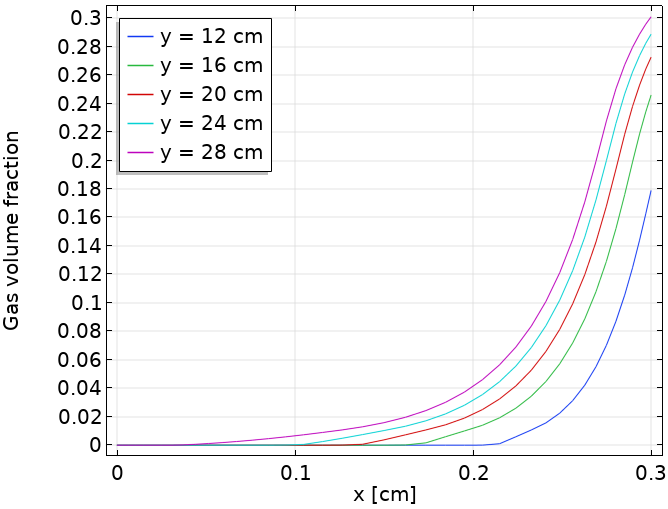
\includegraphics[width=1\linewidth]{volumefraction3mm1000Anosaff.png}
  \caption{The volume fraction profiles in a $0.3 \, \mathrm{cm}$ channel, $i_{av}=1000 \, \mathrm{A/m^2}$}
\end{subfigure}
\begin{subfigure}{.5\textwidth}
  \centering
  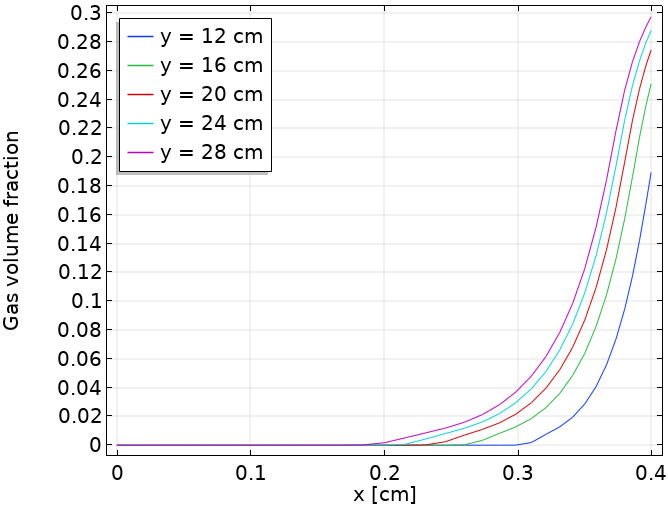
\includegraphics[width=1\linewidth]{volumefraction4mm1000Anosaff.png}
  \caption{The volume  fraction profiles in a $0.4 \, \mathrm{cm}$ channel, $i_{av}=1000 \, \mathrm{A/m^2}$}
\end{subfigure}%
\begin{subfigure}{.5\textwidth}
  \centering
  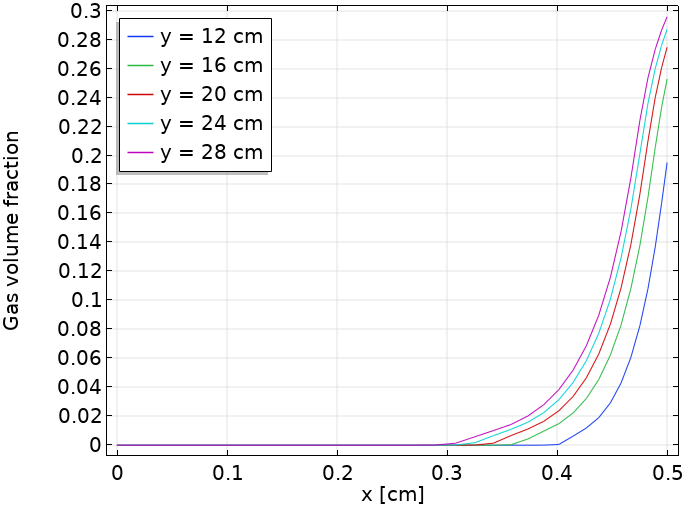
\includegraphics[width=1\linewidth]{volumefraction5mm1000Anosaff.png}
  \caption{The volume fraction profiles in a $0.5 \, \mathrm{cm}$ channel, $i_{av}=1000 \, \mathrm{A/m^2}$}
\end{subfigure}
\caption{The volume fraction profiles in channels with different width $W$ excluding the Saffman lift force, in each of the figures there are 5 profiles obtained at 5 different heights, $y = 12 \, \mathrm{cm}$, $y = 16 \, \mathrm{cm}$, $y = 20 \, \mathrm{cm}$, $y = 24 \, \mathrm{cm}$, $y = 28 \, \mathrm{cm}$}
\label{nosaffvolume}
\end{figure}

However, what the profiles in figure \ref{volumedifferentchannel} and figure \ref{nosaffvolume} have in common is that there seems to be a plateau where the volume fraction gradient decreases, this phenomenon is more noticeable when the current density is higher, as shown in figure \ref{currentdensitycomparison}. Note that in this study, we did not implement any maximum value of volume fraction like the one discussed in equation \ref{eq:coalescencebarrier}. The emergence of the plateau is because the local hydrodynamic self-diffusion velocity increases with volume fraction, which increases with the current density. More detailed discussions can be found in equation \ref{eq:plume4}.






\paragraph{Volume fraction profile under different current densities}
\*


By tuning various parameters, we found that the plume thickness is more influenced by the bubble diameter and viscosity. For example, it is found that the plume thickness is proportional to the bubble diameter. However, since, in reality, the bubble diameter is usually an unchangeable parameter, here we focus on analyzing the influence of channel width and current density on the plume thickness.

From figure \ref{currentdensitycomparison}, we can see the plume thickness is largely independent of the current density; this holds even when there is a noticeable "plateau," like in figure \ref{largecurrentdensity}. As for channel width, it only influences the plume thickness when its value is small. Here we define the bubble plume thickness analogous to the momentum boundary layer: the distance between the gas-evolving wall and where $\alpha_d ( \Bar{x} = \Bar{\delta}) = 0.01\alpha_0$. $\alpha_0$ is the volume fraction at the wall, and plot them in figure \ref{plumethickness} as a function of the channel width. We can see from the figure that channel width and current density only influence the plume thickness when the channel width is small. As the channel width increases, the bubble plume thickness under different conditions all converges to a single value around $1.8 \, \mathrm{mm}$.

\begin{figure}[H]
\centering
\begin{subfigure}{.5\textwidth}
  \centering
  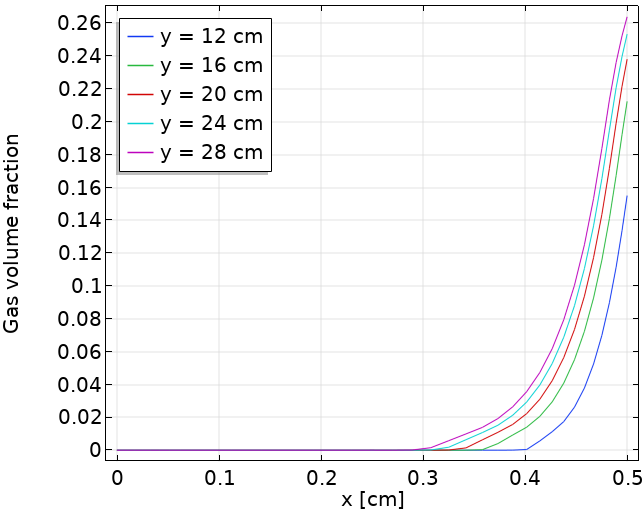
\includegraphics[width=1\linewidth]{volumefractionprofilenosaff5mm800A.png}
  \caption{The volume fraction profiles in a $0.5 \, \mathrm{cm}$ channel, $i_{av}=800 \, \mathrm{A/m^2}$}
\end{subfigure}%
\begin{subfigure}{.5\textwidth}
  \centering
  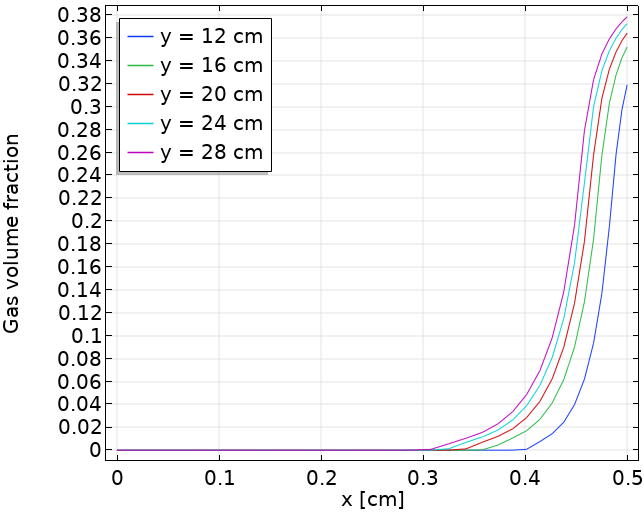
\includegraphics[width=1\linewidth]{volumefractionprofilenosaff5mm2000A.png}
  \caption{The volume fraction profiles in a $0.5 \, \mathrm{cm}$ channel, $i_{av}=2000 \, \mathrm{A/m^2}$}
\end{subfigure}
\begin{subfigure}{.5\textwidth}
  \centering
  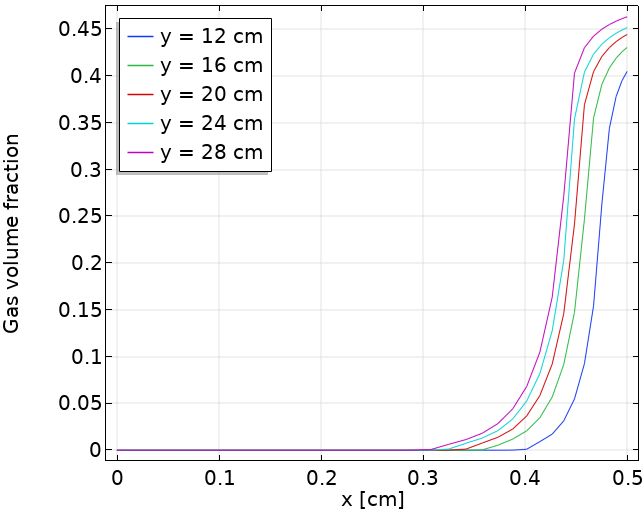
\includegraphics[width=1\linewidth]{volumefractionprofilenosaff5mm4000A.png}
  \caption{The volume fraction profiles in a $0.5 \, \mathrm{cm}$ channel, $i_{av}=4000 \, \mathrm{A/m^2}$}
\end{subfigure}%
\begin{subfigure}{.5\textwidth}
  \centering
  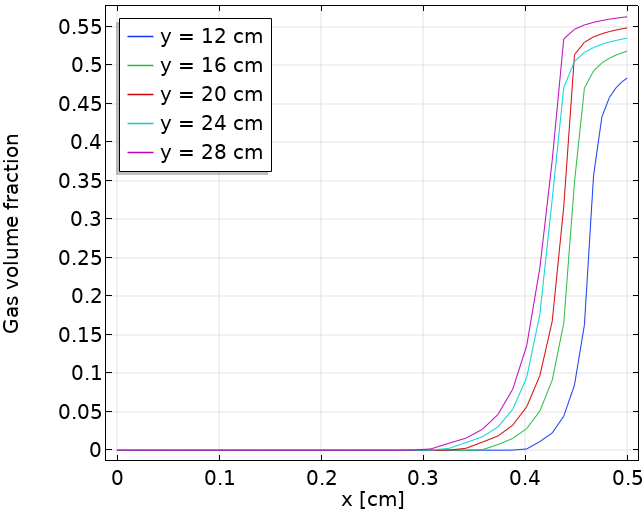
\includegraphics[width=1\linewidth]{volumefractionprofilenosaff5mm8000A.png}
  \caption{The volume fraction profiles in a $0.5 \, \mathrm{cm}$ channel, $i_{av}=8000 \, \mathrm{A/m^2}$}
  \label{largecurrentdensity}
\end{subfigure}
\caption{The volume fraction profiles in a $0.5 \, \mathrm{cm}$ channel with different current densities, in each of the figures there are 5 profiles obtained at 5 different heights, $y = 12 \, \mathrm{cm}$, $y = 16 \, \mathrm{cm}$, $y = 20 \, \mathrm{cm}$, $y = 24 \, \mathrm{cm}$, $y = 28 \, \mathrm{cm}$}
\label{currentdensitycomparison}
\end{figure}



\begin{figure}
    \centering
    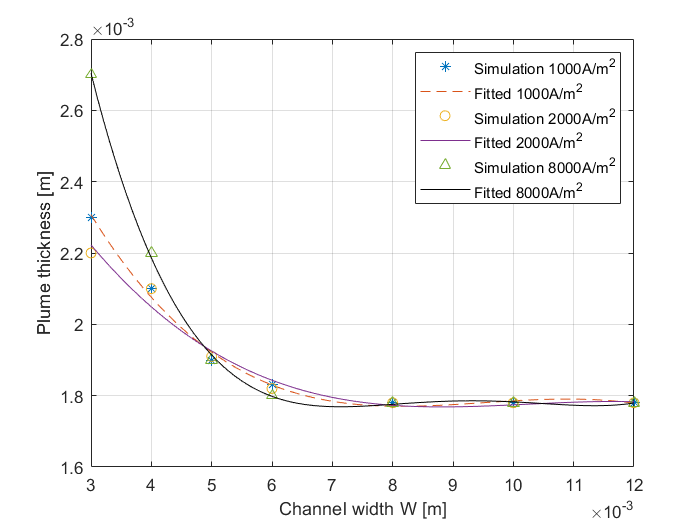
\includegraphics[scale=0.7]{plumethickness.png}
    \caption{The bubble plume thickness as a function of channel width under three different current densities, note that the fitted curves here are merely for visualization purpose, they are simple polynomial fittings. Also note that here the plume thickness at $y = 28 \, \mathrm{cm}$ is recorded as the characteristic plume thickness; each data point stands for one channel, while in figure \ref{plumevsheight} the shown data represents the local plume thickness at different heights in one channel}
    \label{plumethickness}
\end{figure}

\begin{figure}
    \centering
    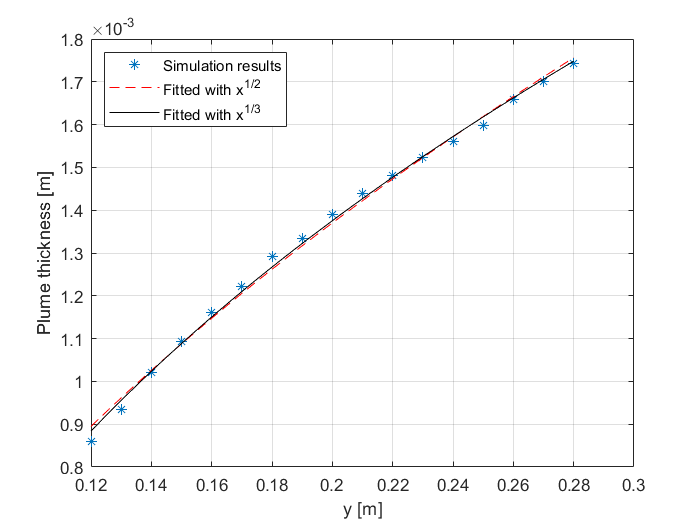
\includegraphics[scale = 0.7]{plumevsheight.png}
    \caption{The bubble plume thickness plotted as a function of height in a $0.5 \, \mathrm{cm}$ channel, $i_{av} = 1000 \, \mathrm{A/m^2}$, two fitted results are also showed as a comparison, it is found that the seems that the two fitting results rarely differs}
    \label{plumevsheight}
\end{figure}

The correlations derived by Schillings et al. \cite{Schillings2015} presented in equation \ref{eq:plumecorrelation} was not found in the simulation of circulation flow in this work. The reason could be that in the circulating channel, the flow velocity is intertwined with many variables, including channel width, current density, bubble diameter, viscosity, and density. In Schillings' work, an inlet liquid velocity is fed at the bottom of the channel (further discussions on why this is still acceptable as the buoyancy-driven flow can be found in Appendix \ref{appendixb}), and gases are evolved from both sides of the wall.  Also, no backflow is found in their simulation, which could be the reason why they can exclude $u_{cy}$ from their correlation.

Here we also try deriving a correlation based on the analogy with thermal and momentum boundary layer by introducing a bubble dispersion coefficient \cite{Schillings2015}, the plume thickness here is taken as a constant, with its value recorded at the top of the channel ($y = 28  \, \mathrm{cm}$):

\begin{equation}\label{eq:plume1}
    \delta_{\alpha} = \sqrt{\frac{\mathcal{D_{\alpha}}H}{u_{cy}}}
\end{equation}

The dispersion coefficient could be scaled as $u_{dx}\delta_{\alpha}$, as the $u_{cx} \sim 0$ at the near wall region, we have $u_{dx} \sim u_{slipx}$. Therefore, the dispersion coefficient has the following scaling law:

\begin{equation}\label{eq:plume2}
    \mathcal{D_{\alpha}} \sim  \delta_{\alpha} u_{slipx}
\end{equation}

From equation \ref{eq:slipmodel} we know that after excluding the Saffman lift force the slip velocity in the x-direction can be scaled with:

\begin{equation}\label{eq:plume3}
    u_{slipx} \sim D_e |u_{Stokes}| /\delta_{\alpha} + D_e^2 u_{cy} \mathfrak{f}(\alpha_d) /\delta_{\alpha}^2 
\end{equation}

Where $\mathfrak{f}(\alpha_d)$ is a function that increases with the local volume fraction. Substitute equation \ref{eq:plume3}, \ref{eq:plume2} into equation \ref{eq:plume1} we have:

\begin{equation}\label{eq:plume4}
    \delta_{\alpha} \sim \sqrt{\frac{D_e^3 \rho_c g H}{18\mu_c u_{cy}}+\frac{D_e^2 H \mathfrak{f}(\alpha_d)}{\delta_{\alpha}}}
\end{equation}

As we can see, this correlation is rather complex; the main challenge is that the condition for scaling bubble plume thickness could be split into four cases: low current density with low and high channel width, and high current density with low and high channel width. 

From figure \ref{plumethickness}, we know that in wider channels the plume thickness remains constant, However, in narrower channels, we only managed to find a trend from figure \ref{plumethickness}, where the bubble plume thickness slightly increases with increasing current density and decreasing channel width. Additionally, figure \ref{plumevsheight} shows that it seems valid to scale plume thickness $\delta_{\alpha}$ with $\sqrt{H}$ as shown in equation \ref{eq:plume4}, though the scaling with $H^{1/2}$ and $H^{1/3}$ rarely differs. 

No general quantitative relation could be given here because the magnitude ratio of the two terms in equation \ref{eq:plume4} also changes as current density grows. From the description in section \ref{otherforces}, we know that the first term on the right-hand side of equation \ref{eq:plume4} is the hydrodynamic self-diffusion and the second term is the shear-induced diffusion. From the simulation results, it is found that under small current density ($i_{av} < 1000 \, \mathrm{A/m^2}$) the hydrodynamic self-diffusion is significantly larger than the shear-induced diffusion, while under large current density it shows a more complex relation as shown in figure \ref{slipcomparison}.

  \begin{figure}[H]
     \centering
     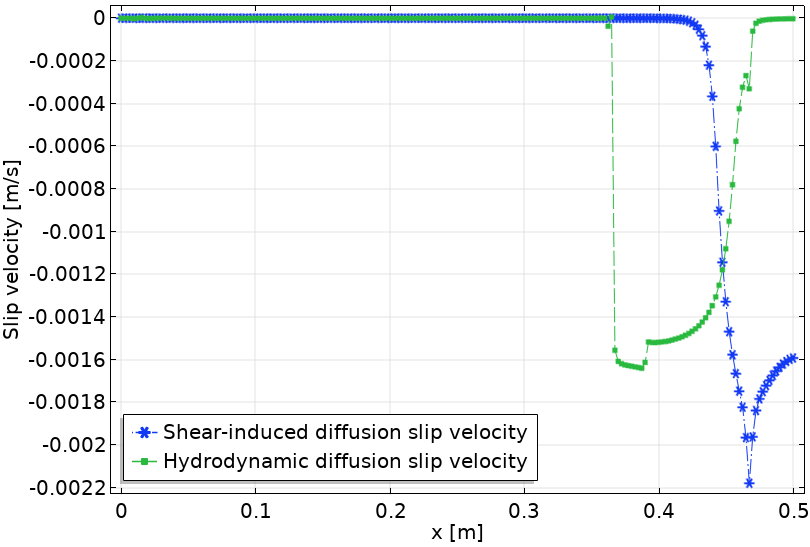
\includegraphics[scale = 0.7]{slipcomparison8000A5mm1.png}
     \caption{Comparison of hydrodynamic slip velocity and shear-induced slip velocity in a $\mathrm{0.5 \, cm}$ channel at $y = 28 \, \mathrm{cm}$ with $i_{av}=8000\, \mathrm{A/m^2}$, the negative velocity values means leftward direction, each mark represents a gridpoint}
     \label{slipcomparison}
 \end{figure}

In figure \ref{slipcomparison} we can see, for a $0.5 \,\mathrm{cm}$ channel, in the first $0.05 \, \mathrm{cm}$ region the shear-induced diffusion dominates, while in the next $0.1 \,\mathrm{cm}$ the hydrodynamic diffusion dominates. While this phenomenon explains why the "plateau" in figure \ref{currentdensitycomparison} becomes more noticeable with larger current density, it also makes it difficult to derive a general scaling law.

\paragraph{Volume fraction profile with turbulent dispersion}
\*

When the liquid phase bulk velocity is large enough, the flow could transit to turbulence \cite{Boissonneau2000}. Currently, there are no clear criteria defining the transition when the bubbles are involved. However, various literature \cite{Rzehak2013, Sokolichin2004} included an additional source term called bubble-induced turbulence. Also, based on the description from Boissonneau et al.\cite{Boissonneau2000}, turbulence were indeed spotted in the vertical channel even under $i_{av} = 500 \, \mathrm{A/m^2}$ for a purely buoyancy-driven flow. Moreover, both turbulent and laminar properties can exist at the same height of the channel, since in their experiments, the turbulent intensity measured at the center of the channel is far less than in the bubbly plume. Therefore, we should assume that the bubbles enhance the turbulence, thus triggering it at a smaller Reynolds number. Normally for channel flow the Criterion for transition to Turbulent flow is $\mathrm{Re}>2300$ \cite{pope2001turbulent}, here we assume the transition happens when $\mathrm{Re}>1500$. 

Here we use the $k-\varepsilon$ model discussed in section \ref{turbulentmodel} to simulate bubbly flow in a $1 \, \mathrm{cm}$ channel under four different current densities as shown in figure \ref{nosaffvolumeturbulent}, the bubble-induced turbulence source term is also included. We assume $\mathrm{Re}$ We can see that the volume fraction profile matches qualitatively with the experimental data from \cite{riegel1998role}.


\begin{figure}[H]
\centering
\begin{subfigure}{.5\textwidth}
  \centering
  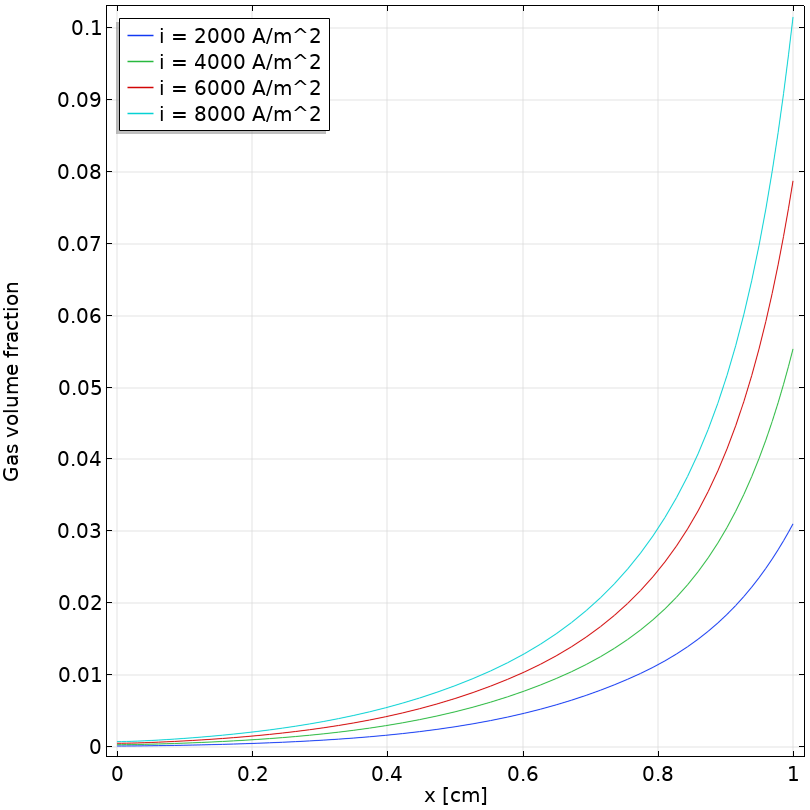
\includegraphics[width=1\linewidth]{volumefractionturbulentcurrentdensitycomparisonnosaff.png}
  \caption{Volume fraction profile at $y = 16 \, \mathrm{cm}$ from turbulent model with different current densities}
\end{subfigure}%
\begin{subfigure}{.5\textwidth}
  \centering
  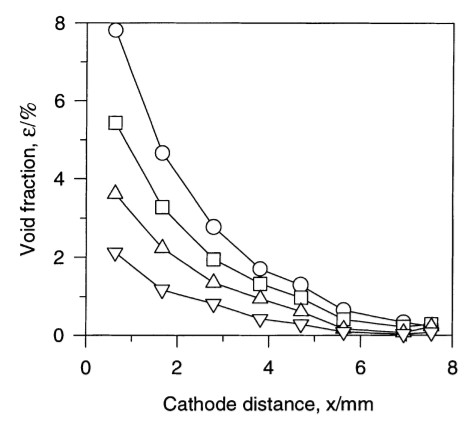
\includegraphics[width=1\linewidth]{profile.png}
  \caption{{volume fraction profile along the channel width \cite{riegel1998role} under different current densities,  $ \nabla: 500 \, \mathrm{A/m^2}, \triangle: 1500 \, \mathrm{A/m^2}, \square: 3250 \, \mathrm{A/m^2}, \bigcirc: 6250 \, \mathrm{A/m^2}$}, an inlet velocity of $0.64 \, \mathrm{m/s}$ is given}
\end{subfigure}
\caption{Comparison of volume fraction profile between $k-\epsilon$ turbulent simulation and experimental data from Riegel et al. \cite{riegel1998role}, the simulation were done in the same setup as before}
\label{nosaffvolumeturbulent}
\end{figure}

  \begin{figure}[H]
     \centering
     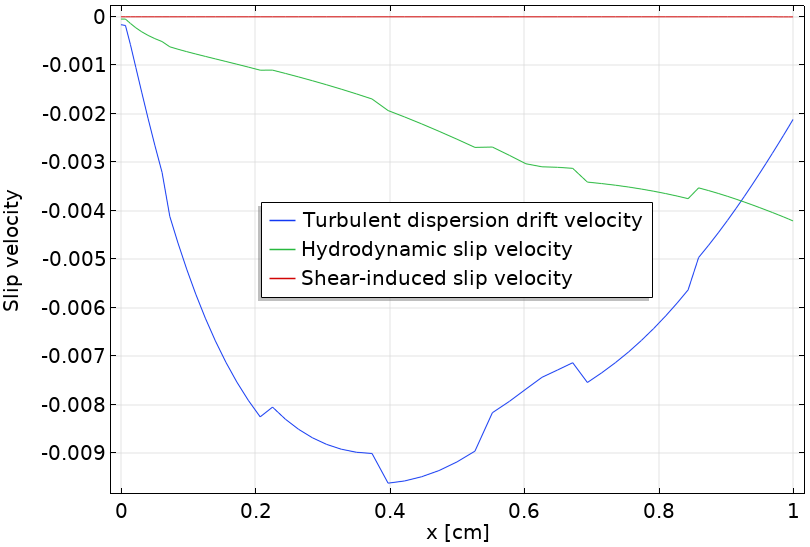
\includegraphics[scale = 0.5]{driftslipcomparison.png}
     \caption{Comparison of hydrodynamic slip velocity shear-induced slip velocity and turbulent drift velocity in a $1 \, \mathrm{cm}$ channel with $i_{av}=6000 \, \mathrm{A/m^2}$, the negative velocity values means leftward direction}
     \label{slipdriftcomparison}
 \end{figure}


  \begin{figure}
     \centering
     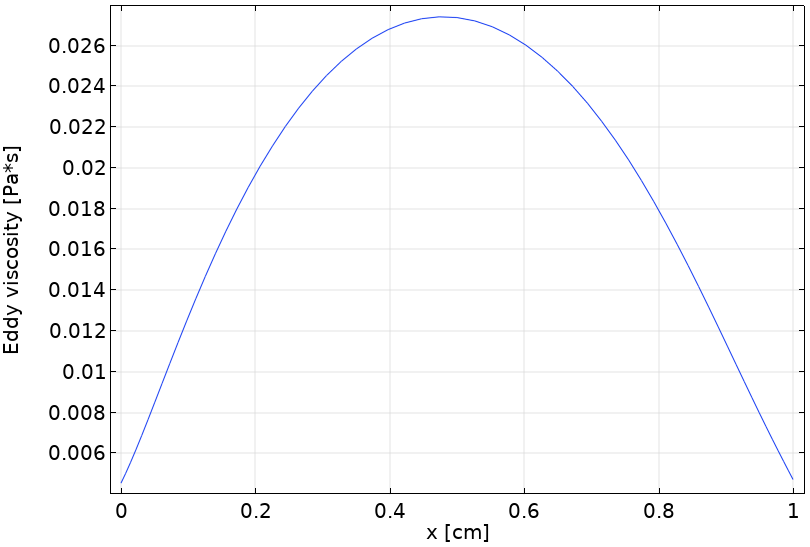
\includegraphics[scale = 0.5]{eddyviscosity.png}
     \caption{The eddy viscosity $\mu_T$ profile in a $1 \, \mathrm{cm}$ channel with $i_{av}=6000 \, \mathrm{A/m^2}$, the negative velocity values means leftward direction}
     \label{eddyviscosity}
 \end{figure}
While the volume fraction is much more uniformly distributed across the channel, the plume thickness is still largely independent of current density. Since the experiment from Riegel et al. \cite{riegel1998role} was done in a $8 \, \mathrm{mm}$ channel with a $0.64 \, \mathrm{m/s}$ inlet velocity at the bottom, we know that $ \mathrm{Re} \sim 6000$, thus the flow should be turbulent. This explains the role of the turbulent dispersion term discussed in section \ref{turbulentmodel}, as in figure \ref{slipdriftcomparison} we can see that in turbulent model the turbulent drift velocity, based on equation \ref{eq:drift}, is several times larger than other two terms, which means the turbulent dispersion could significantly enhance the mixing in the flow field. Interestingly, though eddy viscosity is also based on the volume fraction gradient (see equation \ref{eq:drift}), it does not peak at the near-wall region, this is because the eddy viscosity $\mu_T$ is very small there, as shown in figure \ref{eddyviscosity}.

Another factor different from the laminar flow simulations is that in turbulent flow, even for a large current density, the shear-induced slip velocity is still negligible. This is because, in turbulent models, the use of wall functions keeps the high shear rate within a tiny region near the wall called wall lift-off \cite{COMSOL2016}, in the remaining part of the channel the shear rate remains small, which also keeps the shear-induced diffusion small. Moreover, the fact that the shear rate in the turbulent channel flow is significantly lower makes the correlation for Saffman lift force applicable.


\subsection{Velocity profile across the channel and circulating velocity}

For the velocity profile across the channel and the circulating velocity, we focus on characterizing their relation with the current density and the channel width and try describing them with simple analytical solutions. 


Regarding the velocity, the Saffman lift force only has an indirect influence. Compared with its influence on the volume fraction profile, it does not qualitatively influence the velocity.
Quantitatively, it is found that the results with and without Saffman lift force only differ about 1 to 5 percent depending on the channel width, while in narrower channels, it makes nearly no difference on the velocity profile. 

Additionally, most cases do not satisfy the criteria for the Saffman lift force from equation \ref{eq:shear}. Therefore, we keep using the slip model without the Saffman lift force.




\paragraph{Velocity profile across the channel}
\*

\begin{figure}
\centering
\begin{subfigure}{.5\textwidth}
  \centering
  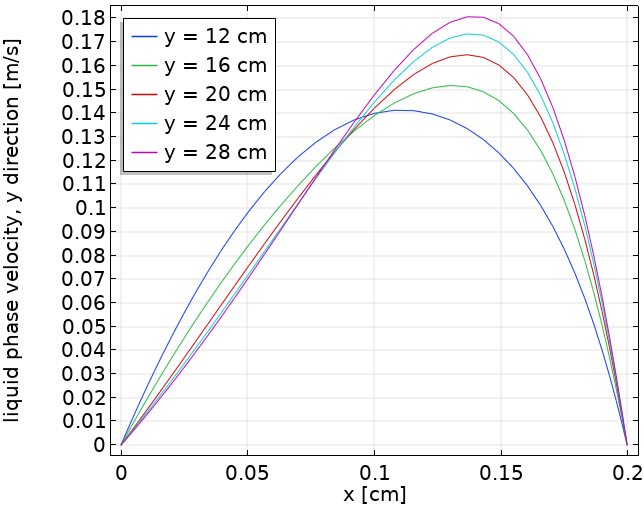
\includegraphics[width=1\linewidth]{velocityprofilenosaff2mm1000A.png}
  \caption{The velocity profiles in a $0.2 \,\mathrm{cm}$ channel, $i_{av}=1000 \, \mathrm{A/m^2}$}
\end{subfigure}%
\begin{subfigure}{.5\textwidth}
  \centering
  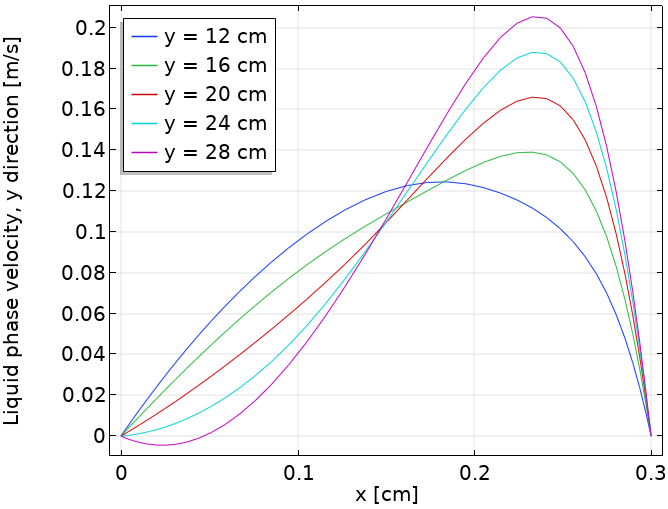
\includegraphics[width=1\linewidth]{velocityprofilenosaff3mm1000A.png}
  \caption{The velocity profiles in a $0.3 \,\mathrm{cm}$ channel, $i_{av}=1000 \, \mathrm{A/m^2}$}
\end{subfigure}
\begin{subfigure}{.5\textwidth}
  \centering
  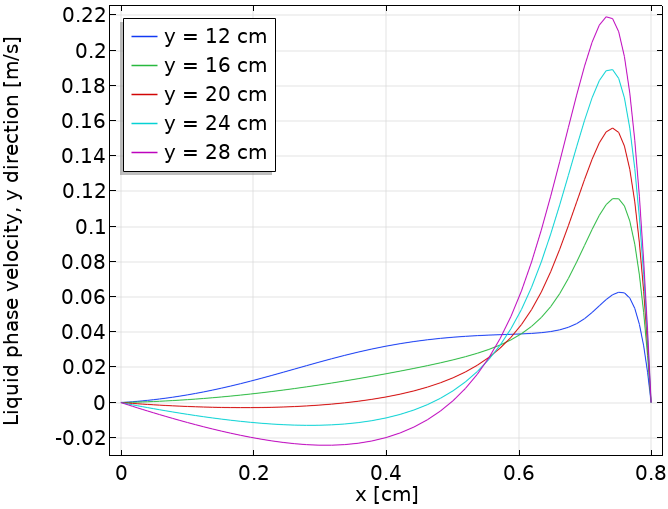
\includegraphics[width=1\linewidth]{velocityprofilenosaff8mm1000A.png}
  \caption{The velocity profiles in a $0.8 \,\mathrm{cm}$ channel, $i_{av}=1000 \, \mathrm{A/m^2}$}
\end{subfigure}%
\begin{subfigure}{.5\textwidth}
  \centering
  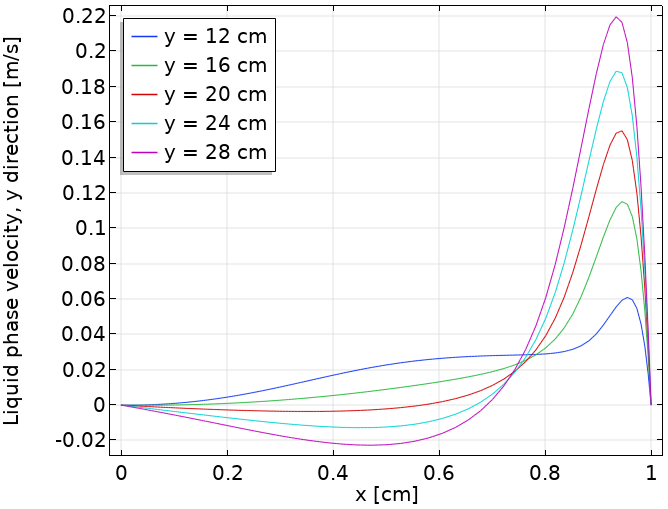
\includegraphics[width=1\linewidth]{velocityprofilenosaff1cm1000A.png}
  \caption{The velocity profiles in a $1 \,\mathrm{cm}$ channel, $i_{av}=1000 \, \mathrm{A/m^2}$}
\end{subfigure}
\caption{The velocity profiles in channels with various width, $i_{av}=1000 \, \mathrm{A/m^2}$, in each of the figures there are 5 profiles obtained at 5 different heights, $y = 12 \, \mathrm{cm}$, $y = 16 \, \mathrm{cm}$, $y = 20 \, \mathrm{cm}$, $y = 24 \, \mathrm{cm}$, $y = 28 \, \mathrm{cm}$}
\label{velocitygapwidthcomparison}
\end{figure}

\begin{figure}
\centering
\begin{subfigure}{.5\textwidth}
  \centering
  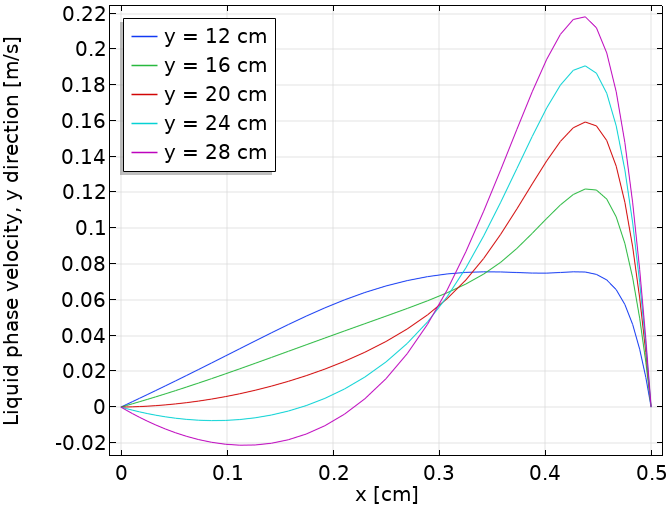
\includegraphics[width=1\linewidth]{velocityprofilenosaff5mm1000A.png}
  \caption{The velocity profiles in a $0.5 \, \mathrm{cm}$ channel, $i_{av}=1000 \, \mathrm{A/m^2}$}
\end{subfigure}%
\begin{subfigure}{.5\textwidth}
  \centering
  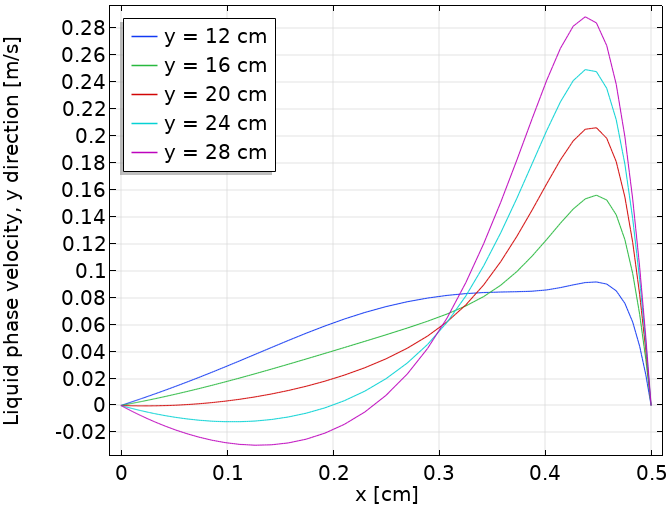
\includegraphics[width=1\linewidth]{velocityprofilenosaff5mm2000A.png}
  \caption{The velocity profiles in a $0.5 \, \mathrm{cm}$ channel, $i_{av}=2000 \, \mathrm{A/m^2}$}
\end{subfigure}
\begin{subfigure}{.5\textwidth}
  \centering
  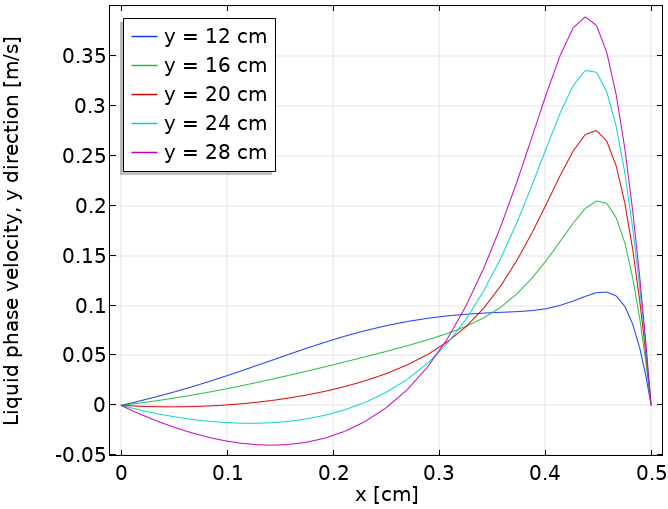
\includegraphics[width=1\linewidth]{velocityprofilenosaff5mm4000A.png}
  \caption{The velocity profiles in a $0.5 \, \mathrm{cm}$ channel, $i_{av}=4000 \, \mathrm{A/m^2}$}
\end{subfigure}%
\begin{subfigure}{.5\textwidth}
  \centering
  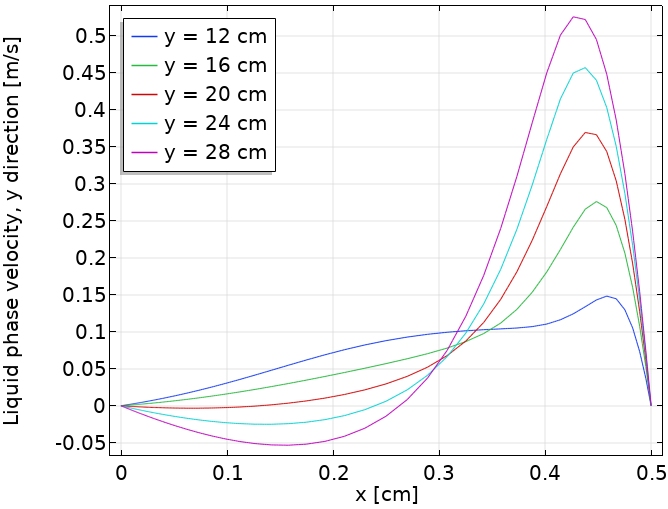
\includegraphics[width=1\linewidth]{velocityprofilenosaff5mm8000A.png}
  \caption{The velocity profiles in a $0.5 \, \mathrm{cm}$ channel, $i_{av}=8000 \, \mathrm{A/m^2}$}
\end{subfigure}
\caption{The velocity profiles in channels with various current densities, in each of the figures there are 5 profiles obtained at 5 different heights, $y = 12 \, \mathrm{cm}$, $y = 16 \, \mathrm{cm}$, $y = 20 \, \mathrm{cm}$, $y = 24 \, \mathrm{cm}$, $y = 28 \, \mathrm{cm}$}
\label{velocitycurrentdensitywithcomparison}
\end{figure}

To characterize the velocity profile with a simple analytical function, we start with using an exponential function to represent the gas volume fraction across the channel \cite{Haverkort2020}:

\begin{equation}\label{eq:analyticalvolumefraction}
    \alpha_d = \alpha_0 e^{-\Bar{x}/(a\Bar{\delta})}
\end{equation}

Where $\alpha_0$ is the volume fraction value at the wall, $\alpha_0$ is a function of $y$, $\Bar{\delta}=\delta / W$ is the dimensionless plume thickness, $\Bar{x}=x/W$ is the dimensionless x coordinates and $a$ is a dimensionless parameter. Here we define the bubble plume thickness analogous to momentum boundary layer: the distance between the gas evolving wall and where $\alpha_d ( \Bar{x} = \Bar{\delta}) = 0.01\alpha_0$. To satisfy this definition, we can make $a = 0.17$ so that $\alpha_d (\Bar{x} = 1) \approx 0.01 $.

This assumed profile could decently represent the volume fraction profile under low current density; for high current density, we can see from figure \ref{currentdensitycomparison} that the volume fraction gradient decreases as it reaches the near-wall region. 

Now, if we look at the velocity profile in channels with different channel width, we can find that as the channel width increases, the velocity profile gradually deviates from the analytical solution of Poiseuille flow. Haverkort \cite{Haverkort2020} used the Navier-Stokes equation without convection terms to describe the velocity profile in the channel, but to include the bubble effect, we can add a corrected hydrostatic pressure term to obtain equation \ref{eq:NSS}.

\begin{equation}\label{eq:NSS}
    0 = \frac{\partial p}{\partial y} +\mu \frac{d^2u_c}{x^2} -(1-\alpha_d)\rho_c g
\end{equation}

Substitute equation \ref{eq:analyticalvolumefraction} into \ref{eq:NSS} we get an analytical solution of velocity profile across the channel \cite{Haverkort2020}:

\begin{equation}\label{eq:velocityanalytical}
    \Bar{u}_d = -\frac{\partial\Bar{p} /\partial \Bar{y}}{2} \Bar{x}(1-\Bar{x}) +\alpha_0 \Bar{\delta}^2a^2(\Bar{x}(e^{-1/(\Bar{\delta}a)}-1)-(e^{-\Bar{x}/(\Bar{\delta}a)}-1))
\end{equation}

Where $\Bar{u}_d = \mu u_{dy}/\rho g W^2$, $\Bar{y} = y/h$, $\Bar{p} = (p + \rho_c g y)/(\rho_c g h)$. Given $W = 5 \, \mathrm{mm}$ we can plot the velocity profile at $y = 28 \, \mathrm{cm}$ as in figure \ref{analyticalcomparison}.

\begin{figure}[H]
\centering
\begin{subfigure}{.45\textwidth}
  \centering
  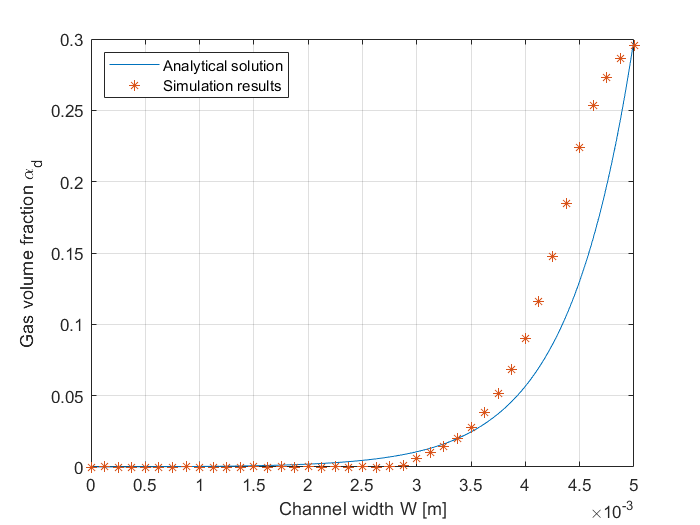
\includegraphics[width=1\linewidth]{volumefractioncomparison.png}
  \caption{The volume fraction profile across the channel, the analytical solution comes from equation \ref{eq:analyticalvolumefraction}}
\end{subfigure}
\begin{subfigure}{.45\textwidth}
  \centering
  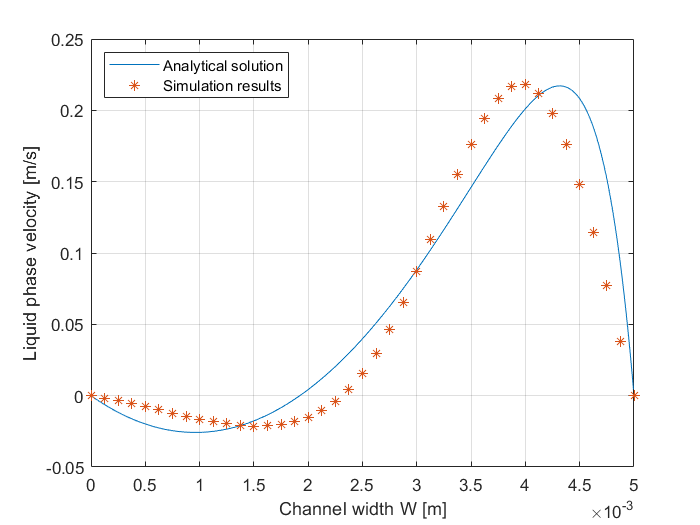
\includegraphics[width=1\linewidth]{Comparisonvelocityprofile.png}
  \caption{The velocity profile across the channel, the analytical solution comes from equation \ref{eq:NSS}}
\end{subfigure}
\caption{Analytical solution in comparison with simulation results in a  $0.5 \, \mathrm{cm} $ channel with 1000 $\mathrm{A/m^2}$, at $y = 28 \, \mathrm{cm}$, $\alpha_0 = 0.3$, $\Bar {\delta}=0.3$, $W= 5\, \mathrm{mm}$, $ \partial \Bar{p}/ \partial \Bar{y} = 0.004$ was used in the analytical solution, while in simulation $ \partial \Bar{p}/ \partial \Bar{y} = 0.003$ }
\label{analyticalcomparison}
\end{figure}

Figure \ref{analyticalcomparison} gives a comparison between the analytical solution and the simulation results. It is found that in a narrower channel, the analytical solution tends to give a decent approximation, while it deviates more from the simulation results as the channel widens. The reason for the deviation could be that in wider channels the velocity profile seems to be independent of the pressure gradient in the y-direction, as the pressure gradient becomes very small after excluding the hydrostatic term ($\partial p/ \partial y \sim 10^{-5} \, \mathrm{Pa \cdot m}$ for channel wider than $1 \,  \mathrm{cm}$). The solution in equation \ref{circulatingvelocity}, however, is always dependent on the pressure gradient.

\paragraph{Backflow in the channel}
\*

Comparing velocity profiles between various channels, we can easily find that the input parameters play a significant role in the size of the backflow. To study this relation, we define the backflow as the distance between the left wall of the channel and the point where the liquid phase velocity equals to zero in the y-direction in the top region of the channel ($ y = 28 \, \mathrm{cm} $, see figure \ref{velocitycontour}), figure \ref{backflowdefinition} gives a sketch for it.

\begin{figure}
    \centering
    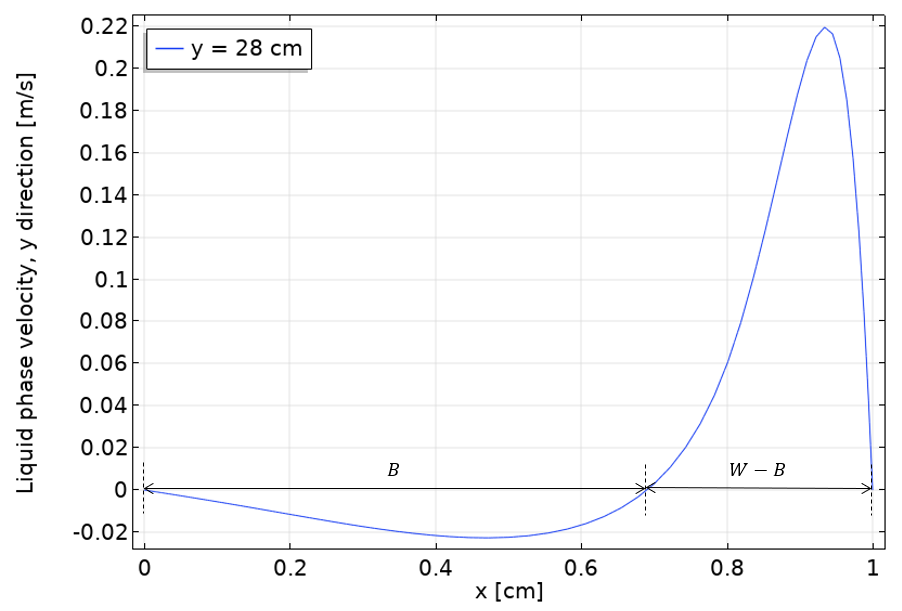
\includegraphics[scale = 0.6]{Backflowdefinition.png}
    \caption{Definition of the backflow size $B$, $(W-B)$ can be interpreted as the range between the right-hand side wall and point where $u_{cy}=0$ in the middle of the channel. Within this range, the velocity profile is still close to Poiseuille flow, we can define it as: $l_b \equiv (W-B)$}
    \label{backflowdefinition}
\end{figure}

Figure \ref{Backflowfit} presents the relation between the backflow size $B$, the current density $i_{av}$ and the channel width $W$, which can also be written as:

\begin{equation}
    B^2 \sim log(i_{av})
\end{equation}

\begin{equation}
    (W-B)^2 \sim W^{\frac{1}{5}}
\end{equation}

While the backflow size is has a pretty explicit logarithmic relation with current density, it is nearly proportional to the channel width. In other words, if the channel width only varies within a limited range, it is safe to estimate $(W-B)$ as a constant.




\begin{figure}[H]
\centering
\begin{subfigure}{.45\textwidth}
  \centering
  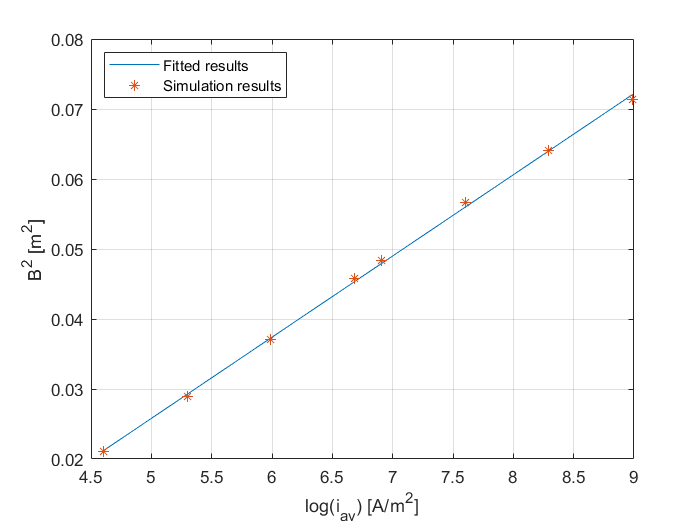
\includegraphics[width=1\linewidth]{backflowfittedwithcurrentdensity.png}
  \caption{The backflow size at $y = 28 \, \mathrm{cm}$ as a function of current density with channel width fixed to $W = 1\, \mathrm{cm}$, $B$ is the backflow size in $\mathrm{m}$, and $i_{av}$ is the current density in $\mathrm{A/m^2}$}
\end{subfigure}
\begin{subfigure}{.45\textwidth}
  \centering
  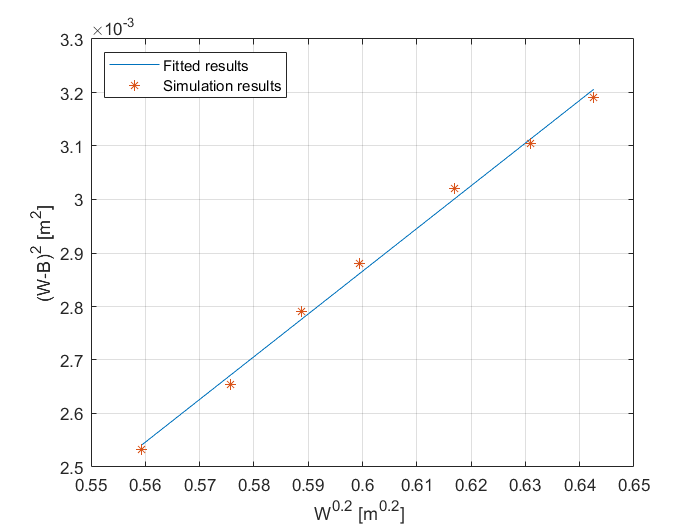
\includegraphics[width=1\linewidth]{backflowfittedwithgapwidth.png}
  \caption{The backflow size at $y = 28 \, \mathrm{cm}$ as a function of riser channel width with current density fixed to $ i_{av} = 1000\, \mathrm{A/m^2}$, $B$ is the backflow size in $\mathrm{m}$, and $W$ is the channel width in $\mathrm{m}$}
  \label{backflow2}
\end{subfigure}
\caption{Backflow size fitted with current density and channel width based on}
\label{Backflowfit}
\end{figure}




\paragraph{Circulating velocity}
\*

In the work of Hine et al. \cite{Hine1980} shown in figure \ref{circulatingvelocity}, the circulating velocity in the riser channel first increases with channel width and then decreases. In this work, similar phenomena are found as well, and the circulating velocity is shown in figure \ref{circulatingvelocityprofile}. 

In very narrow channels ($< 2\, \mathrm{mm}$), the velocity profile is very close to Poiseuille flow; thus, the analytical solution of Poiseuille flow can decently estimate the circulating velocity. Including the volume fraction, it can be written as \cite{Haverkort2020}:

\begin{equation}\label{eq:Poiseulleanalytical}
    \mu_{eff} \frac{\partial^2 u_{cy}}{\partial x^2} = \frac{\partial p}{\partial y} + (1-\langle \alpha_d \rangle) \rho_c g
\end{equation}

Integrating equation \ref{eq:Poiseulleanalytical} two times with no slip boundary condition, we get:

\begin{equation}\label{eq:Poiseuille}
    \langle u_{cy} \rangle =  \frac{W^2}{12\mu_{eff}} (\frac{\partial p}{\partial y} + (1-\langle \alpha_d \rangle)\rho_c g)
\end{equation}

Where $\mu_{eff} = \frac{\mu}{1-\alpha_d}$,  $\langle u_{cy} \rangle$ and $\langle \alpha_d \rangle$ are the average velocity and volume fraction across the channel,. Based on this solution, the circulating velocity should increase with channel width, though it is not proportional with $W^2$ since the volume fraction $\langle \alpha_d \rangle$ will decrease with the increasing channel width. 

However, as the channel width increases, the velocity profile gradually deviates from Poiseuille flow, as shown in figure \ref{velocitygapwidthcomparison}, which makes the equation \ref{eq:Poiseulleanalytical} invalid. Therefore, the solution equation \ref{eq:Poiseuille} also becomes invalid.

An attempt is made to improve the solution from equation \ref{eq:Poiseuille} for a better approximation of the circulating velocity in wider channels. 

From figure \ref{velocitygapwidthcomparison} we can see, the velocity in the top region of the channel stays positive within a certain range as the channel width increases, and within this range, the velocity profile is still close to the Poiseuille flow. From figure \ref{backflow2} we know that this range is a very weak function of the channel width. Therefore, here we define this range as a fixed lengthscale $l_b \equiv (W-B) \approx 3 \mathrm{mm}$, and integrate equation \ref{eq:Poiseulleanalytical} from 0 to $l_b$ instead of $W$ to estimate the flow rate, then we divide it with the channel width $W$ to estimate the average velocity $\langle u_l \rangle$:

\begin{equation}\label{eq:altanalytical}
    \langle u_l \rangle = \frac{\int_0^{l_b} u_{cy}dx}{W} = \langle u_{cy} \rangle =  \frac{l_b^3 (1-\langle \alpha_d \rangle)}{12\mu W} (\frac{\partial p}{\partial y} + (1-\langle \alpha_d \rangle)\rho_c g)
\end{equation}

In this solution, $\langle u_l \rangle$ decreases within an increasing $W$, though it is not perfectly proportional to $1/W$, since $\langle \alpha_d \rangle$ is still changing with channels width.

\begin{figure}[H]
    \centering
    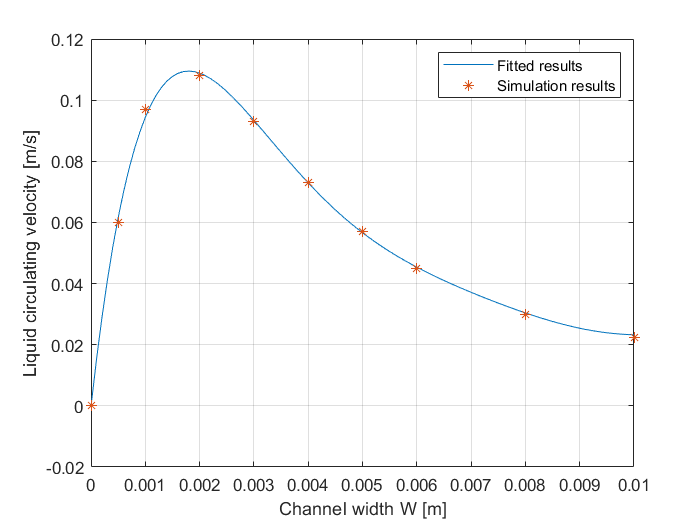
\includegraphics[scale = 0.7]{circulatingvelocityprofile.png}
    \caption{Circulating velocity as a function of channel width $W$, the circulating velocity is calculated as the average velocity across the channel at the $y = 28 \, \mathrm{cm}$, $i_{av} = 1000 \, \mathrm{A/m}$, note that the fitted curve is merely for visualization purpose, they are simple polynomial fittings}
    \label{circulatingvelocityprofile}
\end{figure}


\begin{figure}[H]
    \centering
    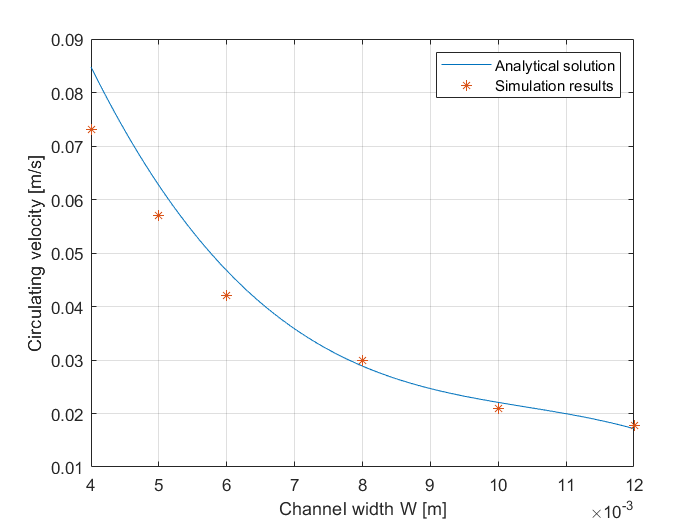
\includegraphics[scale = 0.7]{circulatingcomparison.png}
    \caption{Circulating velocity as a function of channel width $W$ in comparison with the analytical solution from equation \ref{eq:altanalytical}, the current density in the plot is $1000 \, \mathrm{A/m^2}$, the value of $\partial p/ \partial y$ and $\langle \alpha_d \rangle$ all comes from simulation}
    \label{circulatingcomparison}
\end{figure}

Using the solution from equation \ref{eq:altanalytical}, we can again plot the fluid velocity as a function of channel width in comparison with the simulation data in figure \ref{circulatingcomparison}. From the figure, we can find that the analytical solution decently predicts the velocity in wider channels, while in narrower channels, it tends to overestimate the circulating velocity.